\section{Future Work}
\label{sec:future-work}

Elephant Agent opens five concrete research and product directions.

\begin{figure}[t]
  \centering
  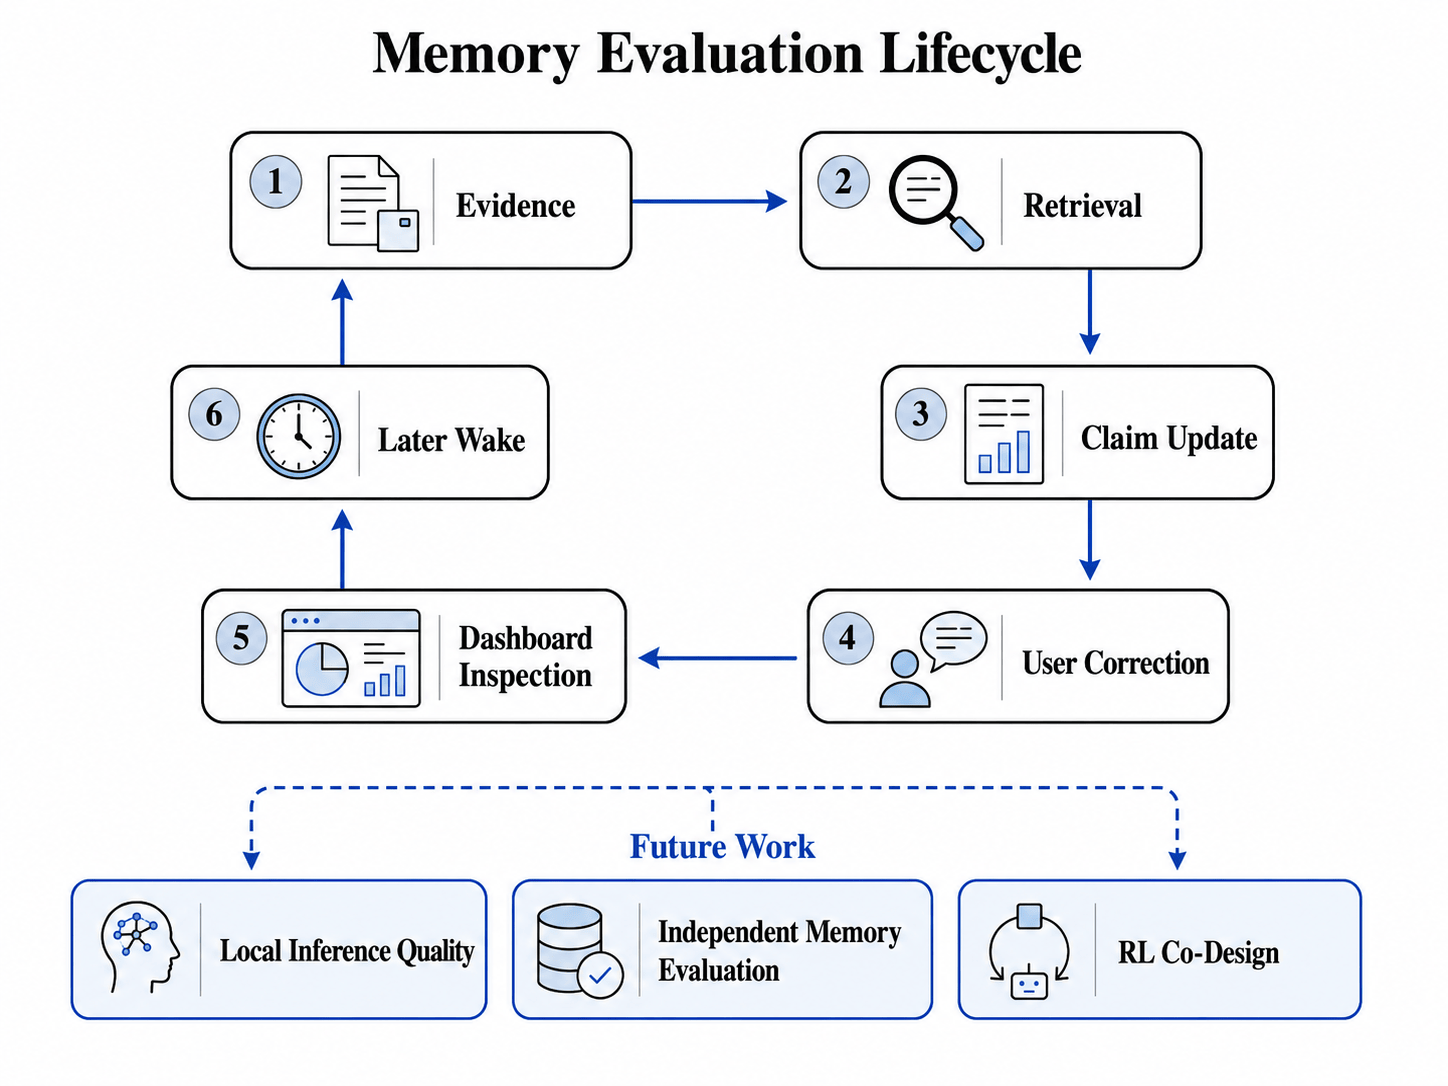
\includegraphics[width=0.9\linewidth]{../../apps/site/static/assets/resources/paper-3.png}
  \caption{Memory evaluation should measure the full lifecycle: evidence,
  retrieval, claim update, user correction, dashboard inspection, and later wake
  behavior, with future work focused on local inference quality, independent
  memory evaluation, and co-design with routing and inference systems.}
  \label{fig:memory-evaluation-lifecycle}
\end{figure}

First, local inference should become faster and more semantically reliable.
The current local path uses a compact sentence-transformers model with
64/256/768 dimensional retrieval modes. Future work should improve latency,
multilingual hybrid recall quality, time-aware ranking calibration,
stance-aware matching, claim-local query expansion, and robustness under
long-running local indexes while keeping active prompt truth in Personal Model
facts.

Second, memory evaluation should become independent of generic chat quality.
Useful benchmarks should measure wake recovery, correction latency, Personal
Model maturity, no-match calibration, social and risk recall, background
learning precision, and whether later answers improve without overriding user
corrections. The evaluation unit should be a lifecycle: evidence, retrieval,
claim update, user correction, dashboard visibility, and later wake behavior.

Third, background skill learning should grow beyond affinity estimation.
Skill affinity is only the first signal: it tells the system which existing
skills fit the user's work and style. A mature background learner should also
notice repeated workflows in the Step trail, propose new user-owned skills when
history reveals a stable pattern, and suggest refinements to existing skills
when evidence shows that a procedure is brittle, stale, or missing local
context. This should remain governed by provenance and operator visibility: the
system may propose or improve skill material, but durable skills should be
inspectable and correctable rather than hidden adaptations.

Fourth, the security boundary should become a first-class research surface.
Personal-model-first agents combine long-lived understanding with tools, code
execution, messaging bridges, and background jobs. Future work should harden
coding sandbox isolation, tool access control, permission scoping, secret
handling, audit trails, and policy checks that decide which tools a foreground
or background agent may call. The important unit is not only a single tool
invocation, but the whole path from recalled support to model decision to tool
execution to durable write.

Fifth, memory should be co-designed with routing, inference, and reinforcement
learning rather than optimized as an isolated retrieval feature. The end-to-end
path is:

\begin{center}
\texttt{agent -> router -> inference -> train}
\end{center}

The routing layer should learn when a turn needs Personal Model search,
conversation search, local embedding, a stronger model, a safer model, or no
recall at all. This naturally connects to vLLM Semantic Router: route by memory
need, language, latency, privacy posture, jailbreak risk, tool-access risk,
confidence, and model-collaboration shape rather than by model cost alone. It
also connects to the vLLM inference engine: local and served inference should
expose latency, batching, cache, and KV-cache optimization signals so Elephant
Agent can choose the right recall and generation posture per turn.

The training side of this co-design is RL post-training over the full agent
lifecycle. The target is not only better tool use or higher task completion.
Training signals should reward asking at the right time, refusing weak memory
support, preserving user corrections, choosing when to write or not write a
claim, selecting the right search surface, using skills only when they fit the
current Personal Model and consent context, and routing through the right model
and inference posture for the user's privacy and safety constraints.
